\chapter{Background}
\label{cap:background}

\section{Stato dell'arte}
\label{sec:stato-dell-arte}

Al momento della scrittura di questa tesi non sono stati trovati dispositivi validati scientificamente in grado di riconoscere le attività di lavaggio e sanificazione delle mani tramite comuni strumenti indossabili. L'unico sistema disponibile commercialmente è SureWash, prodotto dalla GLANTA Ltd, che è in grado di riconoscere i movimenti delle mani dello staff di un ospedale partendo da dati video, ma è limitato al solo riconoscimento di alcuni degli step suggeriti dalla WHO.
Il rilevamento dei movimenti delle mani utilizzando sistemi video è stato studiato da diversi autori, per esempio Zhong et al. nel 2020 hanno proposto un sistema multi-camera in grado di riconoscere sette azioni specifiche legate all'igiene delle mani\cite{zhong2020multi}; più recentemente, Yue et al. sono stati in grado di identificare correttamente sette passaggi del metodo prescritto da alcuni ospedali utilizzando uno strumento di machine learning pre-addestrato chiamato YOLO v3\cite{yue2021intelligent}.
Purtroppo uno dei problemi più grandi di questi sistemi è la privacy, per funzionare infatti richiedono l'installazione di molteplici videocamere in diverse stanze.

Un approccio ortogonale si concentra sul riconoscimento delle attività di lavaggio delle mani tramite sensori inerziali (IMU). In questo ambito è presente un numero ridotto di contributi scientifici, molti dei quali si basano sul utilizzo di molteplici sensori ad alta sensitività e accuratezza, tipici degli strumenti scientifici\cite{galluzzi2015hand}\cite{bal2017system}\cite{li2018wristwash}. 
Anche se le IMU non acquisiscono dati video è comunque importante tenere in considerazione i problemi di privacy, infatti, molti autori hanno mostrato come sia possibile estrarre informazioni chiave riguardanti l'identità dell'utilizzatore partendo dai dati non processati degli accelerometri\cite{jain2018gender}\cite{van2019systematic}.

Queste ricerche preliminari mostrano che il riconoscimento automatico delle attività di lavaggio delle mani attraverso sensori inerziali (accelerometro e giroscopio) è possibile, ma, non approfondiscono le potenzialità degli smartwatch disponibili commercialmente e nemmeno l'applicazione di tecniche di deep learning moderne.

A partire dal 2015 ad oggi sono stati pubblicati solo alcuni lavori rilevanti che fanno uso di smartwatch commerciali: il primo, presentato da Moldol et al., descrive un sistema di monitoraggio in grado di interagire con un distributore di sapone smart per riconoscere l'inizio della procedura di lavaggio\cite{mondol2015harmony}; nel 2020, Mondol et al. e Banerjee et al. hanno presentato due soluzioni per verificare la conformità delle norme della WHO partendo da segnali di sensori IMU \cite{mondol2020hawad}\cite{banerjee2020hand}; più recentemente, Samyoun et al. hanno presentato un sistema di valutazione del lavaggio delle mani basato su smartphone\cite{samyoun2021iwash}, mentre nel 2021, Wu et al. hanno presentato un sistema autonomo di monitoraggio combinando diverse tecnologie di IoT con videocamere e smart dispenser in grado di dare all'utente feedback sul processo di lavaggio delle mani. Infine nel 2022 Fagert et al.hanno introdotto una nuova modalità di rilevamento del lavaggio delle mani misurando le vibrazioni indotte dall'attività sulla struttura del lavandino\cite{fagert2022clean}.

\section{Algoritmi di Machine Learning}
\label{sec:algoritmi-di-machine-learning}

In questa sezione parliamo in maniera più approfondita degli strumenti di apprendimento automatico presi in esame; in particolare per quanto riguarda gli strumenti di machine learning standard abbiamo valutato la Support Vector Machine (SVM) e l'Ensemble Subspace con K-Nearest Neighbors (ES-KNN), mentre nel campo del deep learning abbiamo considerato una Rete Neurale Convoluzionale (CNN) ed un Long Short-Term Memory (LSTM).

\subsection{Support Vector Machine (SVM)}
\label{ssec:support-vector-machine}

SVM è uno degli algoritmi di machine learning più semplici e più utilizzati tradizionalmente per i problemi di regressione e di classificazione con un numero ridotto di campioni.
Un modello SVM rappresenta i dati in input come dei punti nello spazio, mappati in modo tale che i dati appartenenti alle diverse classi siano separati da un margine ampio. I dati sconosciuti sono inseriti nello stesso spazio e la loro categoria dipende dalla regione in cui cadono.

Formalmente, una SVM costruisce un iperpiano, o un insieme di iperpiani, Figura \ref{fig:svm}, in uno spazio a più dimensioni; intuitivamente una buona separazione si può ottenere dall'iperpiano con la distanza maggiore dal punto del training set più vicino di ognuna delle classi; in generale maggiore è il margine fra questi punti, minore è l'errore di generalizzazione commesso dal classificatore. 

Spesso capita che gli insiemi da distinguere non siano linearmente separabili nello spazio, per questo motivo si tende a mappare lo spazio originale in uno con un numero di dimensioni maggiore attraverso funzioni che vengono definite kernel scelte in base al problema da risolvere.

In questa tesi si è optato per l'utilizzo di un SVM con kernel polinomiale, anche se altri kernel sono stati valutati (lineare, quadratico e gaussiano), ma non hanno raggiunto le sue performance.

\begin{figure}[!htb]
    \centering
    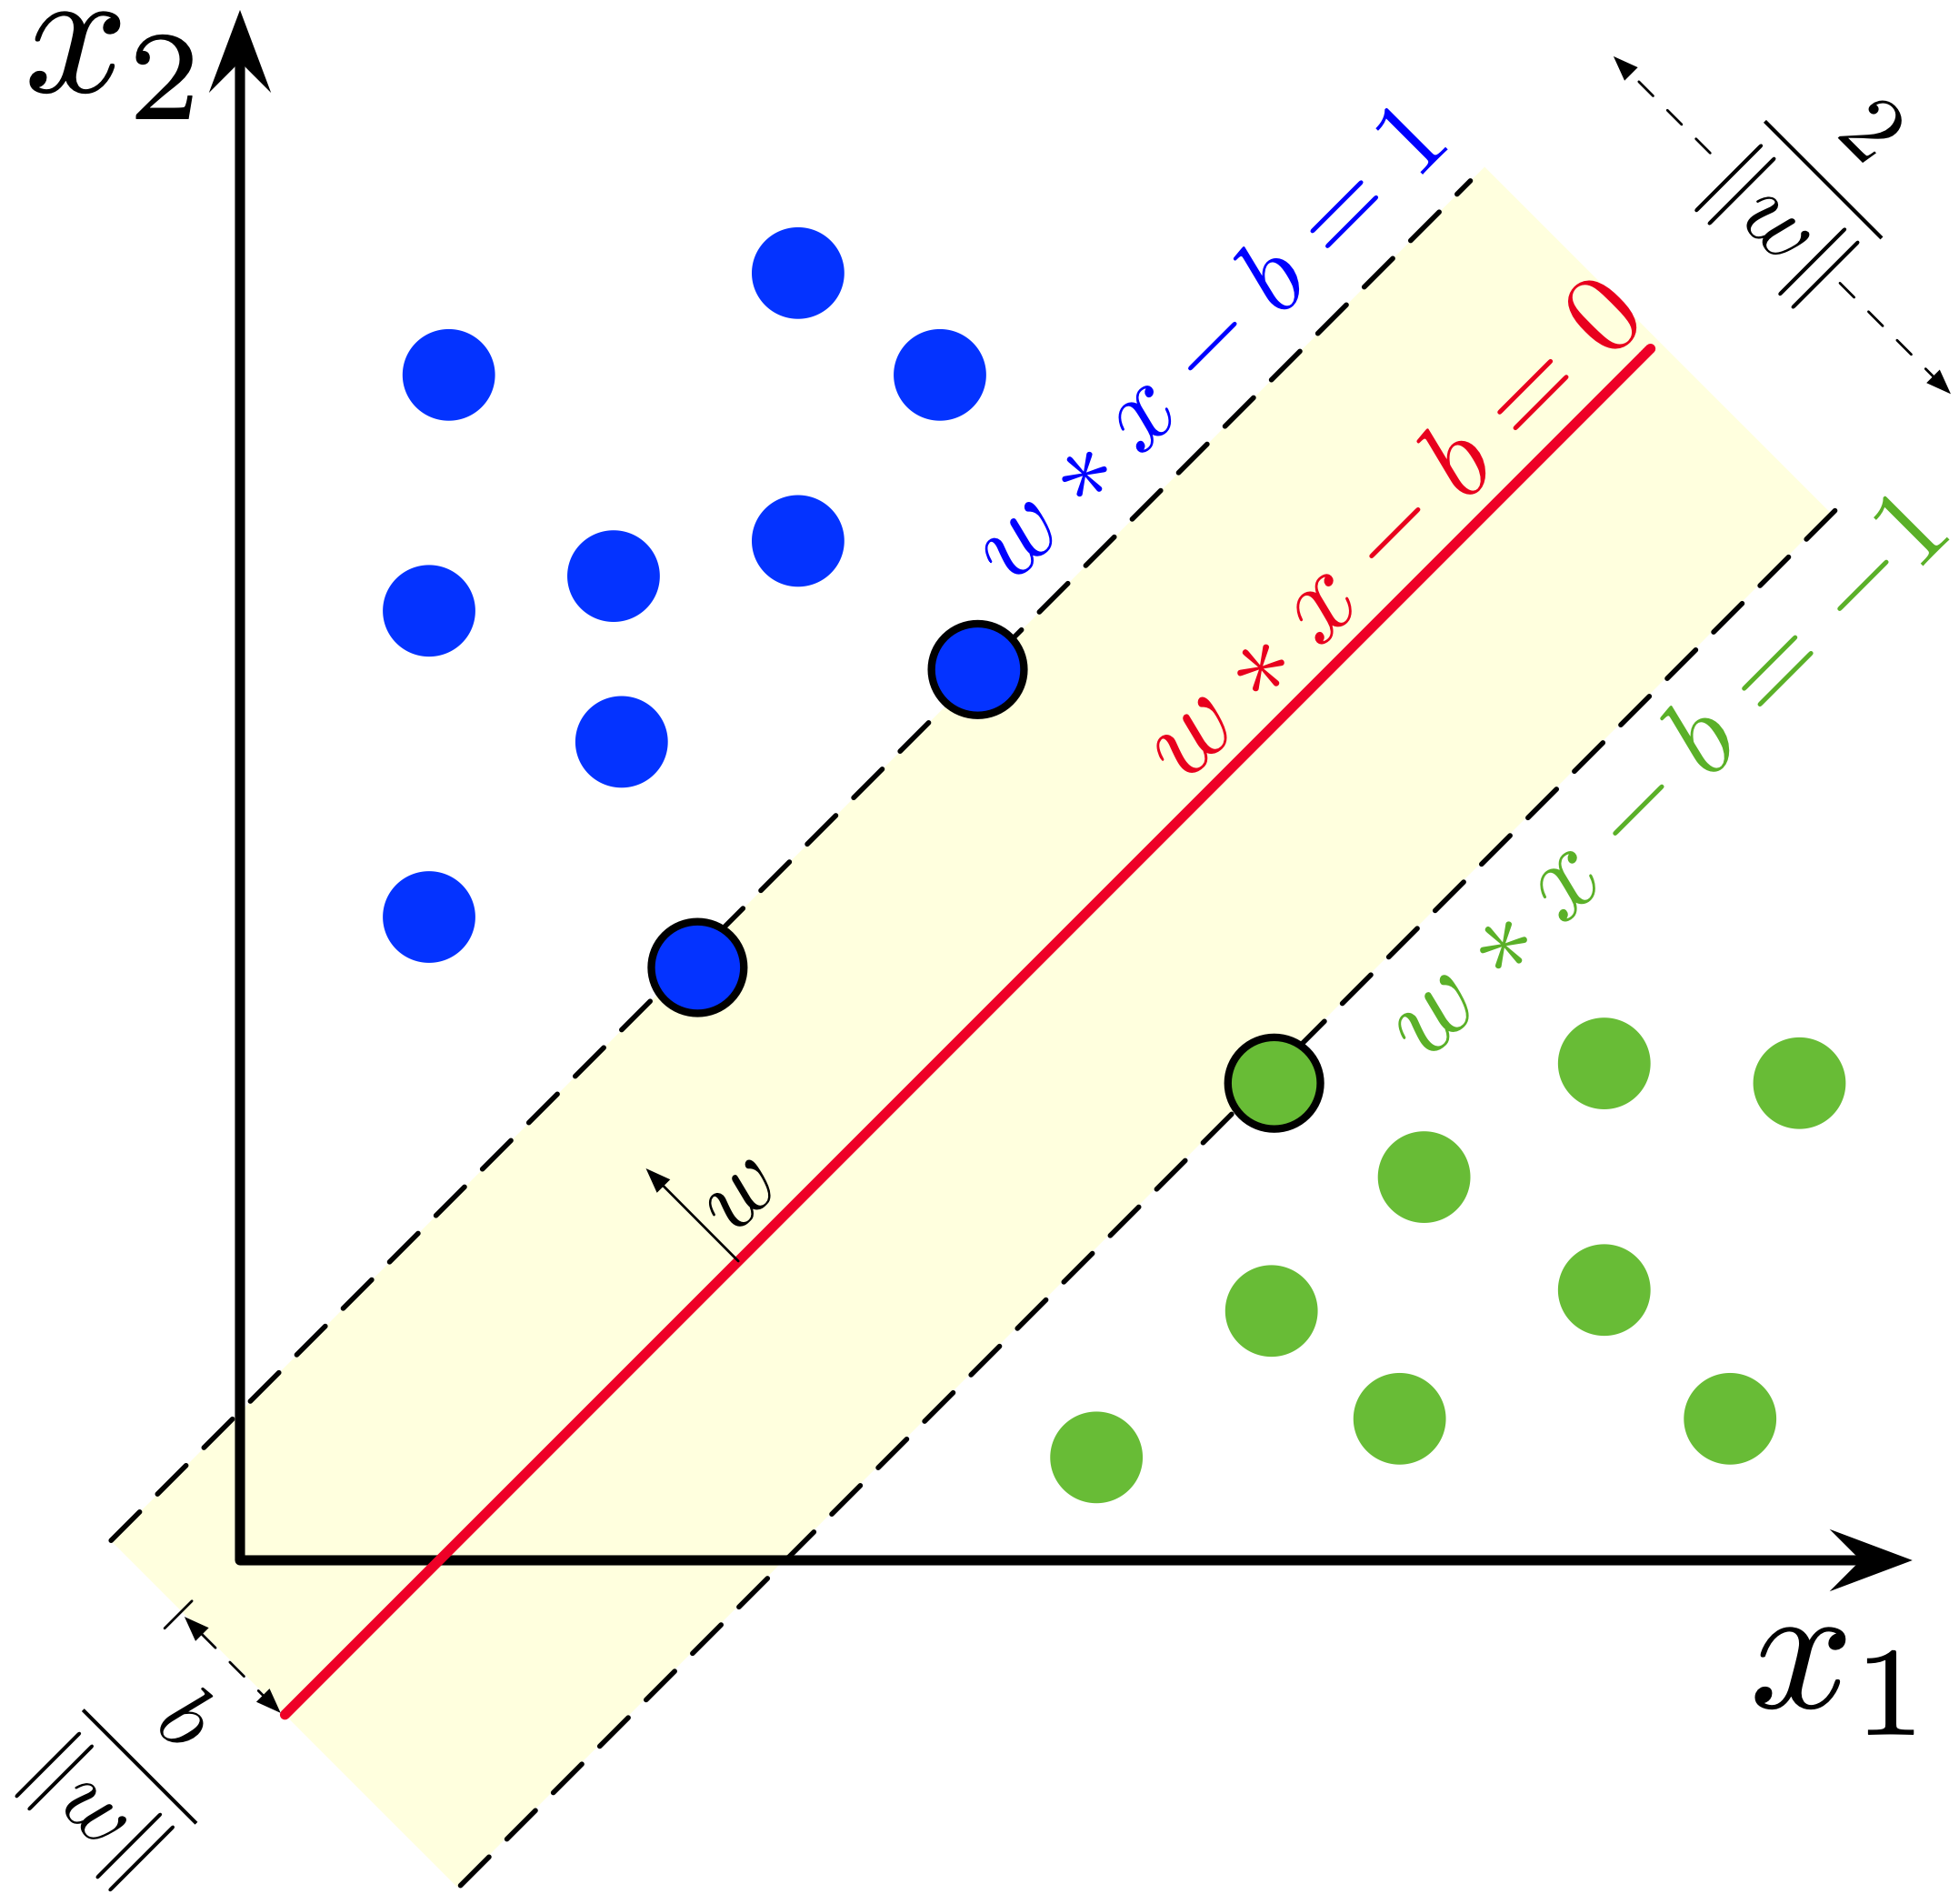
\includegraphics[width=.4\textwidth]{figure/svm.png}
    \caption{Esempio d'iperpiano che meglio separa le due classi di un SVM con kernel lineare.}
    \label{fig:svm}
\end{figure}

\subsection{Ensemble Subspace con K-Nearest Neighbors (ES-KNN)}
\label{ssec:ensemble-subspace-con-knn}

K-Nearest Neighbors (KNN) è un'altro algoritmo di apprendimento automatico molto utilizzato per le sue prestazioni e semplicità. L'algoritmo sfrutta una metrica di distanza per assegnare ad un dato ignoto una classe in base alla maggioranza dei voti dei suoi k vicini. Il parametro k è un intero positivo non molto grande, se k=1 allora l'oggetto viene assegnato alla classe del suo vicino. 

Lo spazio viene partizionato in regioni in base alle posizioni e alle caratteristiche degli oggetti di apprendimento (Figura \ref{fig:knn}), ai fini del calcolo della distanza gli oggetti sono rappresentati attraverso vettori in uno spazio multidimensionale, spesso si usa la distanza euclidea, ma anche altri tipi di distanza sono ugualmente utilizzabili, ad esempio la distanza Manhattan. 
Un punto è assegnato alla classe C se questa è la più frequente fra i k esempi più vicini all'oggetto sotto esame, i vicini sono presi da un insieme di oggetti per cui è nota la classificazione corretta. 

Nonostante la sua semplicità, KNN offre dei risultati competitivi, e in alcuni casi supera di gran lunga altri complessi algoritmi d'apprendimento. Per migliorare le performance di classificazione del KNN nella letteratura sono state proposte delle tecniche di ensemble. In generale le tecniche di ensemble consistono nell'addestrare molteplici modelli per poi combinarli assieme, ad esempio facendo la media, per ottenere l'output desiderato. Un modo per creare un ensemble è quello di addestrare i classificatori con dataset differenti ottenuti suddividendo il training set originario; 
questa tecnica è nota come ensemble subspace. In questa tesi ci concentriamo su una classe di ensemble subspace nota come Ensemble Random Subspace KNN (ERS-KNN) per cui il training set è suddiviso randomicamente nei subspace.

\begin{figure}[!htb]
    \centering
    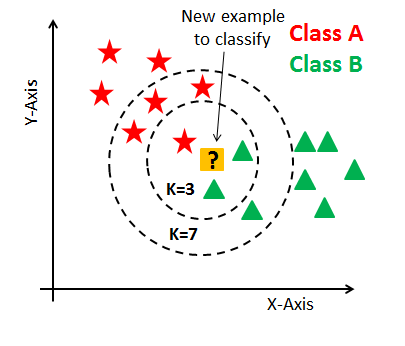
\includegraphics[width=.5\textwidth]{figure/knn.png}
    \caption{Esempio di classificazione di un nuovo dato in un modello KNN binario.}
    \label{fig:knn}
\end{figure}

\subsection{Convolutional Neural Network (CNN)}
\label{ssec:convolutional-neural-network}

CNN(Figura \ref{fig:cnn}) è uno strumento di classificazione dei dati che appartiene alla categoria del deep learning, molto utilizzato negli ultimi anni grazie alla sua struttura che segue un approccio basato sulla computer vision facendo uso delle informazioni spaziali e temporali ricavate dai dati. La struttura della CNN è ispirata dai processi biologici che avvengono nella corteccia visiva degli animali, i cui neuroni sono disposti in maniera tale da rispondere alle regioni di sovrapposizione che tassellano il campo visivo.

Nella pratica CNN è un'estensione di un Multi-Layer Perceptron composto da uno strato di input, vari strati convoluzionali, di pooling e densamente connessi fra loro. Lo strato di input ha il compito di raccogliere i dati sotto forma di pixel di un immagine e passarli agli strati successivi; i livelli convoluzionali sono il nucleo della rete e contengono diversi kernel che convolgono con i dati di input. La convoluzione estrae automaticamente le feature più significative dai dati riducendo la dimensionalità, inoltre l'aggiunta di strati di pooling aiuta a ridurre ulteriormente la dimensione dei parametri andando a fare sub-sampling. Infine uno o più livelli densamente connessi si comportano come un Perceptron tradizionale prendendo le feature in input e producendo una classe in output.

\begin{figure}[!htb]
    \centering
    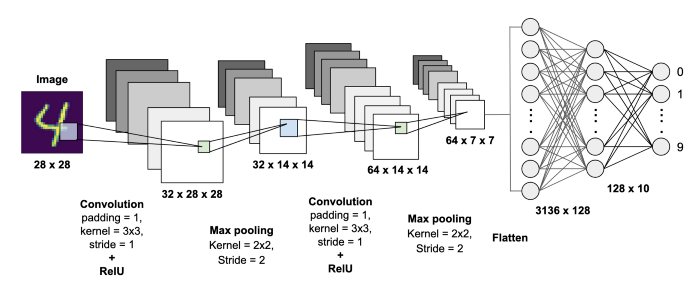
\includegraphics[width=\textwidth]{figure/cnn.png}
    \caption{Esempio della struttura di una rete CNN.}
    \label{fig:cnn}
\end{figure}

\subsection{Long Short-Term Memory (LSTM)}
\label{ssec:long-short-term-memory}

LSTM è una variante delle Reti Neurali Ricorrenti (RNN) utilizzata nel campo del deep learning e dell'intelligenza artificiale per la sua abilità nel classificare e fare predizioni basandosi sui dati delle serie temporali; per questo motivo è spesso usata in ambiti come il riconoscimento della scrittura, il riconoscimento del parlato, la traduzione di testi, il controllo di robot e le applicazioni sanitarie.

Un'unità LSTM(Figura \ref{fig:lstm}) è composta da una cella, un gate di input, un gate di output ed un forget gate; la cella ricorda valori per un tempo arbitrario, mentre i tre gate regolano il flusso delle informazioni dentro e fuori dalla cella prendendo decisioni su cosa ricordare e cosa dimenticare. Il nome LSTM si riferisce al fatto che questo modello ha sia una memoria a lungo termine che una a breve termine, analoga alla struttura del cervello umano.

\begin{figure}[!htb]
    \centering
    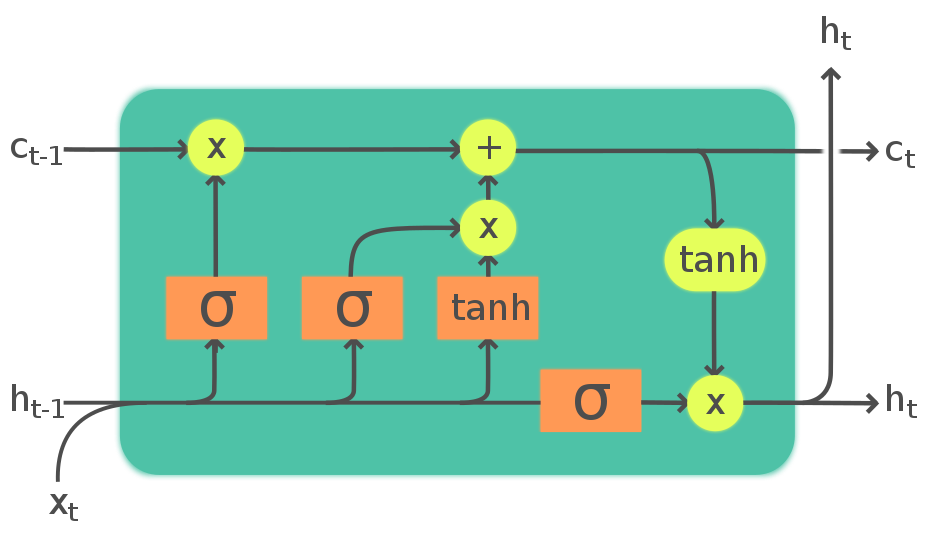
\includegraphics[width=.5\textwidth]{figure/lstm.png}
    \caption{Esempio di una singola unità di una rete LSTM.}
    \label{fig:lstm}
\end{figure}

\section{L'HEXIWEAR}
\label{sec:hexiwear}

Lo smartwatch utilizzato durante la ricerca è l’HEXIWEAR progettato da MikroElektronika in collaborazione con NXP. HEXIWEAR (Figura \ref{fig:hexiwear}) è uno smartwatch completamente open-source dal costo di circa 50\$ che consente lo sviluppo di applicazioni IoT in maniera molto semplice; al suo interno monta ben due MCU: la prima è una Kinetis K64F con architettura ARM Cortex-M4, una frequenza massima di 120MHz, 1024KB di memoria Flash e 256KB di memoria RAM; la seconda è un SoC Kinetis KW40z che permette l’utilizzo delle funzionalità Bluetooth Low Energy. 
All'interno dell'HEXIWEAR sono inoltre presenti una grande quantità di sensori integrati, come ad esempio: 

\begin{itemize}
    \item accelerometro e magnetometro a sei assi FXOS8700
    \item giroscopio a tre assi FXAS21002
    \item sensore di altitudine e pressione MPL3115A2
    \item sensore di temperatura ed umidità HTU21D
    \item sensore di luminosità TSL2561
    \item sensore per il rilevamento dei battiti cardiaci MAX30101
\end{itemize}

Inoltre sono presenti anche un display OLED da 1.1 pollici, una batteria ricaricabile Li-Po da 190mAh e diverse interfacce come: USB, UART, SPI, I2C e SD-card.
Per facilitare lo sviluppo ed il debug delle applicazioni HEXIWEAR ha una docking station al quale è possibile connettere lo smartwatch ed estendere le sue feature con oltre 200 apposite schede dette click boards.

Per sviluppare le applicazioni nell'HEXIWEAR si è deciso di utilizzare la piattaforma MbedOS. Mbed è un sistema operativo real-time open-source creato da ARM per i dispositivi embedded con memoria limitata e che richiedono un basso consumo di corrente. 
Mbed fornisce agli sviluppatori un livello di astrazione tramite il quale possono creare applicazioni IoT scrivendole direttamente in C/C++; esso consiste in un insieme di librerie che forniscono i driver per le periferiche del micro-controllore, l'accesso alla rete, il controllo dell'ambiente RTOS, gli strumenti di build e degli script per test e debug, inoltre è disponibile una repository online dalla quale é possibile scaricare librerie esterne create dalla community.

\begin{figure}[!htb]
    \centering
    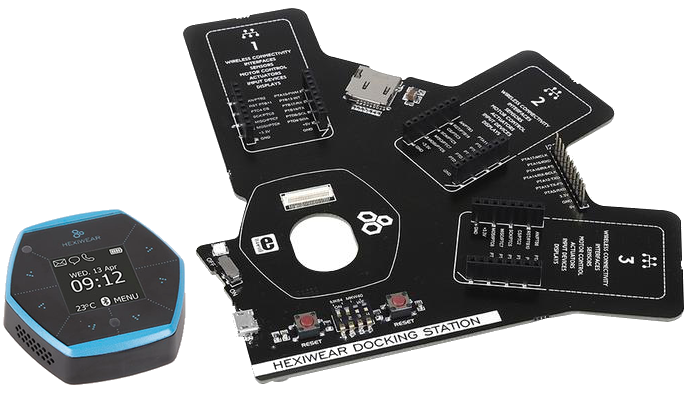
\includegraphics[width=.8\textwidth]{figure/hexiwear.png}
    \caption{HEXIWEAR e la sua docking station.}
    \label{fig:hexiwear}
\end{figure}